\documentclass[12pt,a4paper]{article}

\usepackage[T2A]{fontenc}
\usepackage[utf8]{inputenc}
\usepackage[russian]{babel}
\usepackage[left=2cm,right=2cm,top=2cm,bottom=2cm]{geometry}
\usepackage{amsmath,amssymb}
\usepackage{graphicx}
\usepackage{float}
\usepackage{enumitem}
\usepackage{hyperref}

\emergencystretch=2em

\newcommand{\ran}{\operatorname{ran}}
\newcommand{\rad}{\operatorname{rad}}
\newcommand{\wid}{\operatorname{wid}}
\newcommand{\Mid}{\operatorname{mid}}
\newcommand{\dist}{\operatorname{dist}}
\newcommand{\Mag}{\operatorname{mag}}
\newcommand{\cut}{\operatorname{cut}}
\newcommand{\inter}{\operatorname{int}}
\newcommand{\bfx}{\mathbf{x}}
\newcommand{\bfy}{\mathbf{y}}
\newcommand{\bff}{\mathbf{f}}

\begin{document}

% ======================= Титульный лист =======================
\begin{titlepage}
\begin{center}
Санкт-Петербургский политехнический университет Петра Великого\\
Физико-механический институт\\
Высшая школа прикладной математики и вычислительной физики

\vspace{4cm}

Направление подготовки\\
«01.03.02. Прикладная математика и информатика»

\vspace{3cm}

{\LARGE Дисциплина «Интервальный анализ»}\\[0.5cm]
{\large Отчет по лабораторной работе №2. Вариант № 8}\\[0.3cm]
{\large «Сравнение точности методов интервального оценивания»}
\end{center}

\vspace{3cm}

\begin{flushright}
\begin{minipage}{0.35\textwidth}
\textbf{Работу выполнил:}\\
Фамилия И. О.\\
Группа:\\
5030102/?????
\end{minipage}
\end{flushright}

\vfill
\begin{center}
Санкт-Петербург\\
2026
\end{center}
\end{titlepage}

\tableofcontents
\newpage

% ======================= 1. Постановка задачи =======================
\section{Постановка задачи}

\textbf{Цель работы:} исследование и сравнение точности различных методов интервального оценивания областей значений функций одной и нескольких переменных; изучение влияния формы функционального выражения, выбора центра и дробления интервального бруса на качество получаемых оценок.

\textbf{Задачи.}
\begin{enumerate}
\item Для функций одной переменной $f_1(x)=x^3-3x^2+2$ на $X=[0,3]$ и $f_2(x)=x^4-5x^2+4$ на $X=[-1,2]$:
  \begin{enumerate}[label=\Alph*.]
  \item найти точную область значений $\ran(f,X)$ и построить график;
  \item вычислить интервальные оценки области значений: естественное интервальное расширение (B.1), форму Горнера или другое алгебраически эквивалентное выражение (B.2), дифференциальную центрированную форму с разными центрами (B.3), наклонную центрированную форму (B.4), бицентрированную форму по теореме Баумана (B.5);
  \item для каждой оценки вычислить расстояние $\dist(F,\ran)$; найти константы Липшица (C.1), получить теоретические оценки полуширины (C.2) и сравнить с ними $\rad F(X)$ (C.3).
  \end{enumerate}
\item Для функции двух переменных $f_3(x,y)=x^2+2xy+2y^2-3x+y$ на брусе $X=[-1,2]\times[-2,1]$:
  \begin{enumerate}[label=E.\arabic*]
  \item построить поверхность и линии уровня;
  \item найти точную область значений;
  \item вычислить естественное интервальное расширение;
  \item вычислить естественные расширения алгебраически эквивалентных выражений;
  \item вычислить дифференциальную центрированную форму с разными центрами;
  \item вычислить бицентрированную форму;
  \item исследовать влияние дробления бруса пополам по $x$ и по $y$;
  \item получить покоординатную липшицевскую оценку;
  \item сравнить все оценки с $\ran(f_3,X)$.
  \end{enumerate}
\end{enumerate}

\textbf{Выбор интервала для $f_2$.} Производная $f_2'(x)=4x^3-10x=2x(2x^2-5)$ обращается в нуль в точках $x=0$ и $x=\pm\sqrt{5/2}\approx\pm1.5811$, вторая производная $f_2''(x)=12x^2-10$ "--- в точках $x=\pm\sqrt{5/6}\approx\pm0.9129$. Нули функции: $f_2(x)=(x^2-1)(x^2-4)=0$ при $x=\pm1,\pm2$. Выбран интервал $X=[-1,2]$: он содержит локальный максимум $x=0$ ($f_2(0)=4$), локальный минимум $x=\sqrt{5/2}$ ($f_2=-2.25$) и обе точки перегиба $x=\pm0.9129$. На $X$ функция $f_2$ возрастает на $[-1,0]$, убывает на $[0,\sqrt{5/2}]$ и снова возрастает на $[\sqrt{5/2},2]$; на концах $f_2(-1)=f_2(2)=0$. Интервал несимметричен и содержит нуль внутри себя, что существенно для формы Горнера (п.~B.2).

% ======================= 2. Теоретическая часть =======================
\section{Теоретическая часть}

\subsection*{Интервальные оценки}

\textbf{Интервальное расширение} "--- интервальная функция $\bff$, совпадающая с $f$ на вырожденных интервалах и монотонная по включению: $\bfx\subseteq\bfy\Rightarrow\bff(\bfx)\subseteq\bff(\bfy)$. Для любого интервального расширения $\ran(f,X)\subseteq\bff(X)$.

\textbf{Оптимальное интервальное расширение:} $\bff^{*}(X)=\square\,\ran(f,X)$ "--- интервальная оболочка области значений.

\textbf{Естественное интервальное расширение} получается заменой аргументов на интервалы, а операций и элементарных функций "--- на их интервальные аналоги. Интервальная арифметика рассматривает каждое вхождение переменной как независимую величину, поэтому при многократных вхождениях оценка завышается: например, $X-X=[-\wid X,\wid X]$, а не $0$; $[-1,1]\cdot[-1,1]=[-1,1]$, тогда как $[-1,1]^2=[0,1]$. Если каждая переменная входит в выражение один раз, естественное расширение совпадает с оптимальным.

\textbf{Формы интервального оценивания:}
\begin{itemize}
\item \textbf{Дифференциальная центрированная (среднезначная) форма:}
\[
F_{mv}(X,c)=f(c)+\bff'(X)(X-c),\qquad c\in X,
\]
где $\bff'(X)$ "--- интервальная оценка производной (в работе "--- её естественное расширение). Для функции нескольких переменных $F_{mv}(X,c)=f(c)+\sum_i \bff'_{x_i}(X)(X_i-c_i)$. Включение $\ran(f,X)\subseteq F_{mv}(X,c)$ следует из теоремы Лагранжа.

\item \textbf{Наклонная центрированная форма:}
\[
F_{sl}(X,c)=f(c)+\bff^{\angle}(X,c)(X-c),
\]
где $f^{\angle}(x,c)=\dfrac{f(x)-f(c)}{x-c}$ при $x\neq c$, $f^{\angle}(c,c)=f'(c)$ "--- наклон. По теореме Лагранжа $f^{\angle}(x,c)=f'(\xi)$ для некоторой точки $\xi$ между $x$ и $c$, поэтому множество наклонов содержится в $\ran(f',X)$, и наклонная форма, как правило, уже дифференциальной.

\item \textbf{Бицентрированная форма:}
\[
F_{bic}(X)=F_{mv}(X,c_{*})\cap F_{mv}(X,c^{*})=\bigl[\,\underline{F_{mv}(X,c_{*})},\ \overline{F_{mv}(X,c^{*})}\,\bigr],
\]
где центры $c_{*}$, $c^{*}$ выбираются по теореме Баумана (см. ниже).

\item \textbf{Форма Горнера} "--- алгебраически эквивалентная запись многочлена
\[
a_nx^n+a_{n-1}x^{n-1}+\dots+a_1x+a_0=(\dots((a_nx+a_{n-1})x+a_{n-2})x+\dots)x+a_0.
\]
Она устраняет сложение и вычитание независимо оценённых степеней (например, $X^3-3X^2$), что часто сужает оценку. Однако степени в ней заменяются произведениями, а $X\cdot X\supsetneq X^2$ при $0\in\inter X$. Поэтому на интервалах, содержащих нуль внутри, форма Горнера может оказаться хуже исходной записи.

\item \textbf{Выделение полного квадрата и разложение на множители} "--- другие эквивалентные преобразования, уменьшающие число вхождений переменной, например $x^4-5x^2+4=\bigl(x^2-\tfrac52\bigr)^2-\tfrac94=(x^2-1)(x^2-4)$. Квадрат вычисляется как степень интервала и оценивается точно.
\end{itemize}

\textbf{Теорема Баумана.} Пусть $\bff'_{x_i}(X)$ "--- интервальные оценки частных производных на $X$ и
\[
p_i:=\cut\!\left(\frac{\Mid\bff'_{x_i}(X)}{\rad\bff'_{x_i}(X)},\,[-1,1]\right),\quad
(c_{*})_i:=\Mid X_i-p_i\rad X_i,\quad (c^{*})_i:=\Mid X_i+p_i\rad X_i,
\]
$i=1,\dots,n$. Тогда среди всех центров $c\in X$:
\begin{itemize}
\item нижняя граница $F_{mv}(X,c)$ максимальна при $c=c_{*}$;
\item верхняя граница $F_{mv}(X,c)$ минимальна при $c=c^{*}$;
\item $\rad F_{mv}(X,c)$ минимален при $c=\Mid X$.
\end{itemize}
Следовательно, $F_{bic}(X)\subseteq F_{mv}(X,c)$ для любого $c\in X$. Если $0\notin\bff'_{x_i}(X)$ для всех $i$ (функция монотонна по каждой переменной), то $p_i\in\{-1,1\}$, центры $c_{*}$, $c^{*}$ совпадают с вершинами бруса $X$ и
\[
F_{mv}(X,c_{*})\cap F_{mv}(X,c^{*})=\square\{f(c_{*}),f(c^{*})\}=\ran(f,X).
\]
В теореме фигурирует функция срезки $\cut:\mathbb{R}\times\mathbb{IR}\to\mathbb{R}$:
\[
\cut(x,[\underline{x},\overline{x}]):=
\begin{cases}
\underline{x}, & \text{если } x<\underline{x},\\
x, & \text{если } x\in[\underline{x},\overline{x}],\\
\overline{x}, & \text{если } x>\overline{x}.
\end{cases}
\]

\textbf{Расстояние между интервалами (метрика Хаусдорфа).} Отображение $\dist:\mathbb{IR}\times\mathbb{IR}\to\mathbb{R}_{+}$, определяемое как
\[
\dist(\mathbf{a},\mathbf{b}):=\max\{|\underline{a}-\underline{b}|,\ |\overline{a}-\overline{b}|\},
\]
задаёт расстояние между интервалами $\mathbf{a}$ и $\mathbf{b}$. В работе оно используется для сравнения полученной оценки $F(X)$ с точной областью значений $\ran(f,X)$: $\dist=0$ означает точное совпадение, чем больше значение, тем сильнее оценка отличается от истины.

\textbf{Порядок приближения.} Для естественного расширения и для центрированных форм соответственно
\[
\dist\bigl(F(X),\ran(f,X)\bigr)=O(\wid X),\qquad
\dist\bigl(F_{mv}(X,c),\ran(f,X)\bigr)=O\bigl((\wid X)^2\bigr).
\]
Поэтому центрированные формы выигрывают у естественного расширения на узких интервалах, а на широких их преимущество не гарантировано.

\subsection*{Липшицевы оценки}

Функция $f$ липшицева на $X$ с константой $L$, если $|f(x)-f(y)|\le L|x-y|$ для всех $x,y\in X$. Для дифференцируемой $f$ по теореме Лагранжа можно взять $L=\max_{x\in X}|f'(x)|$. Тогда
\[
\rad\ran(f,X)\le L\rad X.
\]
Это неравенство относится к области значений (и к оптимальному расширению); интервальная оценка $F(X)\supseteq\ran(f,X)$ может его нарушать.

Интервальное расширение $\bff$ липшицево на $X$ с константой $L_F$, если $\wid\bff(Y)\le L_F\wid Y$ для всех $Y\subseteq X$; тогда $\rad\bff(X)\le L_F\rad X$. Так как $\bff(Y)\supseteq\ran(f,Y)$, всегда $L_F\ge L$. В естественном расширении ширины слагаемых складываются при любом знаке ($\wid(A\pm B)=\wid A+\wid B$), поэтому на малом интервале $Y\ni x$ для многочлена $\sum_k a_kx^k$ имеем $\wid\bff(Y)\approx\bigl(\sum_k k|a_k||x|^{k-1}\bigr)\wid Y$, и $L_F$ равна максимуму этого множителя по $x\in X$.

Для функции двух переменных на брусе $X=X_1\times X_2$ используется покоординатная оценка
\[
\rad F\le L_1\rad X_1+L_2\rad X_2,\qquad
L_1=\sup_{(x,y)\in X}\left|\frac{\partial f}{\partial x}(x,y)\right|,\quad
L_2=\sup_{(x,y)\in X}\left|\frac{\partial f}{\partial y}(x,y)\right|.
\]

% ======================= 3. Реализация =======================
\section{Реализация}

Работа реализована на языке Python~3 с использованием библиотек \texttt{numpy}, \texttt{matplotlib} и \texttt{intvalpy} (класс \texttt{Interval}, функция \texttt{mag}). Код разделён на три модуля:
\begin{itemize}
\item \texttt{calculations.py} "--- функции и их производные, все интервальные оценки, расстояния и константы Липшица;
\item \texttt{plots.py} "--- графики $f_1$, $f_2$ (п.~A), поверхность и линии уровня $f_3$ (п.~E.1);
\item \texttt{results.py} "--- вывод таблиц оценок и расстояний, проверка липшицевых оценок.
\end{itemize}

Особенности реализации:
\begin{itemize}
\item Точные области значений $f_1$ и $f_2$ найдены перебором по равномерной сетке из $10^6$ точек и подтверждены аналитически; для $f_3$ "--- аналитически, с перебором вершин и минимумов на рёбрах бруса (п.~E.2).
\item Для форм $F_{mv}$ и $F_{sl}$ (пп.~B.3, B.4) взято по 11 центров, равномерно расположенных на $X$, включая концы и середину: $c=0,\,0.3,\dots,3$ для $f_1$ и $c=-1,\,-0.7,\dots,2$ для $f_2$.
\item Производные в $F_{mv}$ оцениваются естественным расширением выражений $f_1'(x)=3x^2-6x$ и $f_2'(x)=4x^3-10x$.
\item Наклон нельзя получить подстановкой $X$ в дробь $(f(x)-f(c))/(x-c)$, так как $X-c\ni0$. Поэтому дробь сокращается аналитически. Для $f_1$ коэффициенты частного находятся делением на $x-c$ по схеме Горнера в точке $c$, после чего частное вычисляется на $X$ также по схеме Горнера:
\[
f_1^{\angle}(x,c)=\bigl(x+c-3\bigr)x+c^2-3c.
\]
Для $f_2$ использовано разложение $x^4-c^4-5(x^2-c^2)=(x-c)(x+c)(x^2+c^2-5)$:
\[
f_2^{\angle}(x,c)=(x+c)\bigl(x^2+c^2-5\bigr).
\]
В нём $X^2$ вычисляется как степень (точно), поэтому оценка наклона уже, чем у частного по Горнеру $\bigl((x+c)x+c^2-5\bigr)x+c^3-5c$, содержащего произведения $X\cdot X$ при $0\in\inter X$; второй вариант также вычислен для сравнения.
\item В бицентрированной форме нижняя граница берётся из $F_{mv}(X,c_{*})$, а верхняя "--- из $F_{mv}(X,c^{*})$.
\item Константа $L$ вычисляется как $\max|f'|$ по сетке из $10^6$ точек, константа $L_F$ "--- численно, как $\max\wid\bff(Y)/\wid Y$ по 3000 подынтервалам $Y=[t,t+h]\subseteq X$, $h=10^{-4}$.
\item Расстояние $\dist$ реализовано по определению (совпадает с \texttt{intvalpy.dist}).
\end{itemize}

% ======================= 4. Результаты =======================
\section{Результаты}

Во всех таблицах методы сравниваются по величине $\dist(F,\ran)$ "--- расстоянию между полученной оценкой и точной областью значений. Чем меньше $\dist$, тем ближе оценка к истине. Жирным выделены лучшие значения; числа округлены до трёх знаков после запятой.

\subsection*{Функция $f_1(x)=x^3-3x^2+2$, $X=[0,3]$}

\textbf{A.} Производная $f_1'(x)=3x^2-6x=3x(x-2)$ обращается в нуль при $x=0$ и $x=2$. Сравнивая значения $f_1(0)=2$, $f_1(2)=-2$, $f_1(3)=2$, получаем $\ran(f_1,X)=[-2,2]$, ширина 4; перебор по сетке даёт тот же результат. График функции приведён на рис.~\ref{fig:f1}.

\begin{figure}[H]
\centering
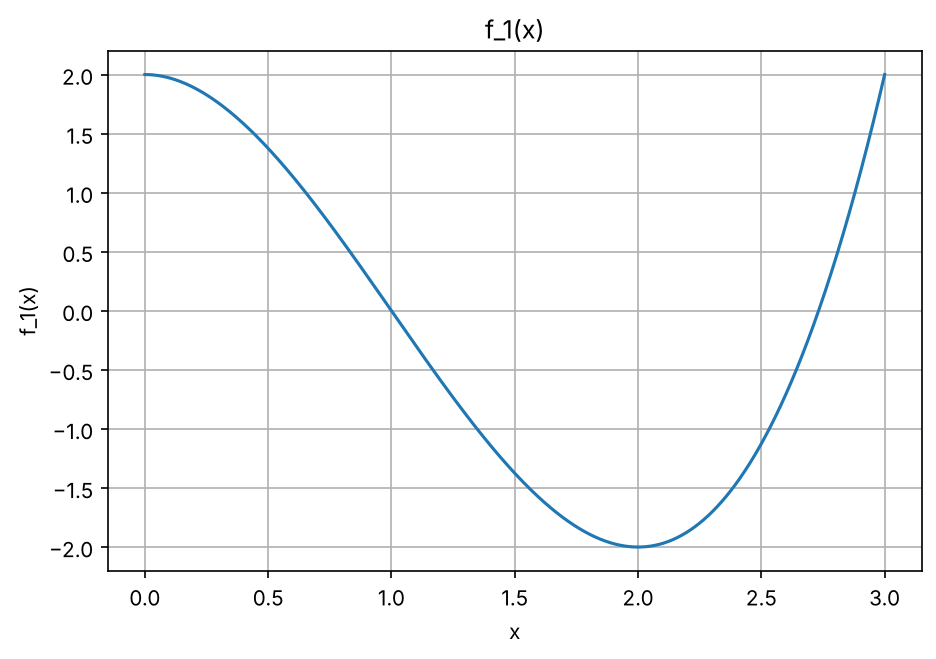
\includegraphics[width=0.6\textwidth]{f1_plot.png}
\caption{График $f_1(x)$ на $X=[0,3]$.}
\label{fig:f1}
\end{figure}

\textbf{B.} Естественное расширение (B.1): $X^3-3X^2+2=[0,27]-[0,27]+2=[-25,29]$. Форма Горнера (B.2): $((X-3)X)X+2=[-25,2]$. Оценка производной для B.3 и B.5: $\bff_1'(X)=3X^2-6X=[-18,27]$, тогда как точная область значений производной на $X$ равна $[-3,9]$. Для бицентрированной формы (B.5) $p=\cut(4.5/22.5)=0.2$, $c_{*}=1.2$, $c^{*}=1.8$. Центрированные формы при разных центрах приведены в табл.~\ref{tab:f1c}, сводное сравнение "--- в табл.~\ref{tab:f1}.

\begin{table}[H]
\centering
\begin{tabular}{|c|c|c|c|c|}
\hline
$c$ & $F_{mv}(X,c)$ & $\dist$ & $F_{sl}(X,c)$ & $\dist$ \\
\hline
0.0 & $[-52.000,\ 83.000]$ & 81.000 & $[-25.000,\ 2.000]$ & 23.000 \\
0.3 & $[-46.843,\ 74.657]$ & 72.657 & $[-22.300,\ 4.430]$ & 20.300 \\
0.6 & $[-42.064,\ 65.936]$ & 63.936 & $[-19.600,\ 6.320]$ & 17.600 \\
0.9 & $[-37.501,\ 56.999]$ & 54.999 & $[-16.900,\ 7.670]$ & 14.900 \\
1.2 & $[-32.992,\ 48.008]$ & 46.008 & $[-14.200,\ 8.480]$ & 12.200 \\
1.5 & $[-41.875,\ 39.125]$ & \textbf{39.875} & $[-11.500,\ 8.750]$ & 9.500 \\
1.8 & $[-50.488,\ 30.512]$ & 48.488 & $[-8.800,\ 8.480]$ & \textbf{6.800} \\
2.1 & $[-58.669,\ 35.831]$ & 56.669 & $[-11.230,\ 7.670]$ & 9.230 \\
2.4 & $[-66.256,\ 41.744]$ & 64.256 & $[-15.280,\ 6.320]$ & 13.280 \\
2.7 & $[-73.087,\ 48.413]$ & 71.087 & $[-19.870,\ 4.430]$ & 17.870 \\
3.0 & $[-79.000,\ 56.000]$ & 77.000 & $[-25.000,\ 2.000]$ & 23.000 \\
\hline
\end{tabular}
\caption{Дифференциальная (B.3) и наклонная (B.4) центрированные формы для $f_1$}
\label{tab:f1c}
\end{table}

\begin{table}[H]
\centering
\begin{tabular}{|l|c|c|c|}
\hline
Метод & $F(X)$ & Ширина & $\dist(F,\ran)$ \\
\hline
\textbf{Наклонная}, $c=1.8$ (лучший центр) & $[-8.800,\ 8.480]$ & 17.280 & \textbf{6.800} \\
Наклонная, $c=1.5=\Mid X$ & $[-11.500,\ 8.750]$ & 20.250 & 9.500 \\
Форма Горнера & $[-25.000,\ 2.000]$ & 27.000 & 23.000 \\
Естественное расширение & $[-25.000,\ 29.000]$ & 54.000 & 27.000 \\
Бицентрированная ($c_{*}=1.2$, $c^{*}=1.8$) & $[-32.992,\ 30.512]$ & 63.504 & 30.992 \\
Дифф. центрир., $c=1.5$ (лучший центр) & $[-41.875,\ 39.125]$ & 81.000 & 39.875 \\
Дифф. центрир., $c=0$ (худший центр) & $[-52.000,\ 83.000]$ & 135.000 & 81.000 \\
\hline
\end{tabular}
\caption{Сравнение методов для $f_1$ ($\ran=[-2,2]$)}
\label{tab:f1}
\end{table}

\textbf{Наблюдения:}
\begin{itemize}
\item \textbf{Лучший результат по $\dist$} "--- наклонная форма при $c=1.8$: $\dist=6.8$; при $c=\Mid X=1.5$ получаем 9.5. Оценка наклона значительно уже оценки производной: при $c=1.5$ $\bff_1^{\angle}(X,c)=[-6.75,2.25]$ против $\bff_1'(X)=[-18,27]$. При каждом из 11 центров $F_{sl}(X,c)\subseteq F_{mv}(X,c)$, а ширина меньше в 3.6--5 раз.
\item \textbf{Форма Горнера} ($\dist=23$) лучше естественного расширения ($\dist=27$): её верхняя граница точная, так как в записи $((x-3)x)x+2$ все множители знакопостоянны на $X$ ($X-3=[-3,0]$, $X=[0,3]$). Нижняя граница $-25$ по-прежнему завышена: значение $-3$ множителя $X-3$ достигается при $x=0$, а значение 3 множителя $X$ "--- при $x=3$. При $c=0$ наклонная форма в точности совпадает с формой Горнера: $F_{sl}(X,0)=2+((X-3)X)X$; при $c=3$ получается тот же интервал $[-25,2]$.
\item \textbf{Естественное расширение} ($\dist=27$): каждая степень оценивается точно ($X^3=[0,27]$, $3X^2=[0,27]$), но при вычитании они рассматриваются как независимые, и ширины складываются.
\item \textbf{Бицентрированная форма} ($\dist=30.992$) лучше любой дифференциальной формы: её нижняя граница $-32.992$ совпадает с нижней границей $F_{mv}(X,1.2)$, а верхняя $30.512$ "--- с верхней границей $F_{mv}(X,1.8)$, и это наилучшие границы в столбце $F_{mv}$ табл.~\ref{tab:f1c}. Однако она хуже естественного расширения.
\item \textbf{Дифференциальные центрированные формы} "--- худшие результаты: от $\dist=39.875$ ($c=1.5$) до 81 ($c=0$). Причина "--- завышенная оценка производной: $\bff_1'(X)=[-18,27]$ (ширина 45) при точной области $[-3,9]$ (ширина 12), и это завышение умножается на $X-c$ ширины 3. Ширина $F_{mv}$ минимальна (81) при всех $c\in[c_{*},c^{*}]=[1.2,1.8]$, в том числе при $c=\Mid X$, что согласуется с теоремой Баумана.
\end{itemize}

\subsection*{Функция $f_2(x)=x^4-5x^2+4$, $X=[-1,2]$}

\textbf{A.} Сравнивая значения в критических точках и на концах интервала, $f_2(-1)=0$, $f_2(0)=4$, $f_2(\sqrt{5/2})=-9/4$, $f_2(2)=0$, получаем $\ran(f_2,X)=[-2.25,\ 4]$, ширина 6.25; перебор по сетке даёт тот же результат. Минимум достигается во внутренней точке $x=\sqrt{5/2}\approx1.5811$, максимум "--- во внутренней точке $x=0$. График приведён на рис.~\ref{fig:f2}.

\begin{figure}[H]
\centering
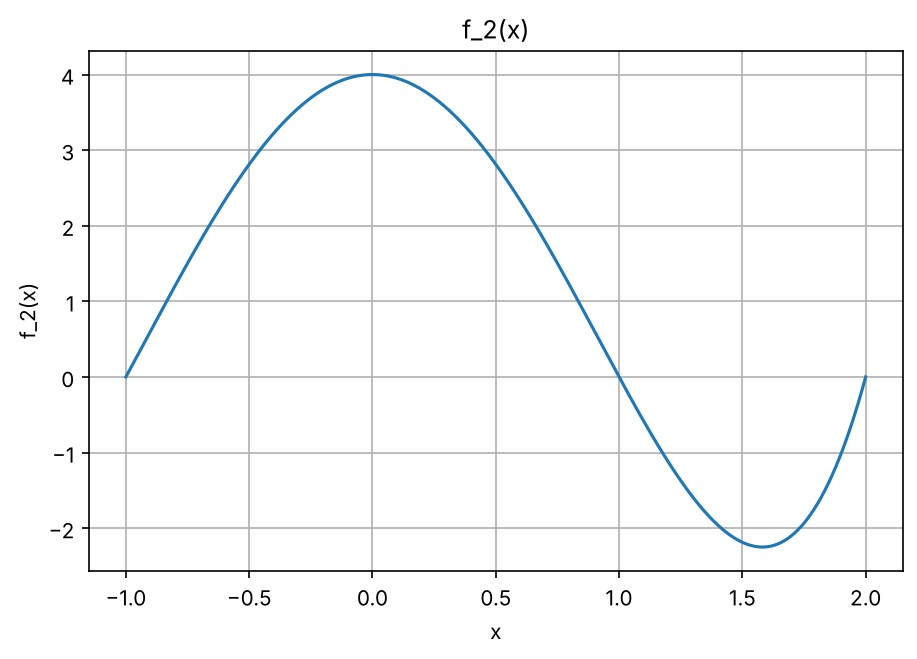
\includegraphics[width=0.6\textwidth]{f2_plot.png}
\caption{График $f_2(x)$ на $X=[-1,2]$.}
\label{fig:f2}
\end{figure}

\textbf{B.} Естественное расширение (B.1): $X^4-5X^2+4=[0,16]-[0,20]+4=[-16,20]$. Схема Горнера для $f_2$ хуже исходной записи: $((X\cdot X-5)X)X+4=[-24,18]$, так как $X\cdot X=[-2,4]$, а $X^2=[0,4]$. Поэтому в п.~B.2 основным взято выделение полного квадрата $f_2(x)=\bigl(x^2-\tfrac52\bigr)^2-\tfrac94$, что даёт $\bigl(X^2-\tfrac52\bigr)^2-\tfrac94=[-2.25,\ 4]$; для сравнения вычислено и разложение на множители $(X^2-1)(X^2-4)=[-1,3]\cdot[-4,0]=[-12,4]$. Оценка производной: $\bff_2'(X)=4X^3-10X=[-24,42]$, тогда как точная область значений производной равна $[-6.086,\ 12]$. Для бицентрированной формы $p=\cut(9/33)\approx0.273$, $c_{*}\approx0.091$, $c^{*}\approx0.909$. Результаты приведены в табл.~\ref{tab:f2c} и~\ref{tab:f2}.

\begin{table}[H]
\centering
\begin{tabular}{|c|c|c|c|c|}
\hline
$c$ & $F_{mv}(X,c)$ & $\dist$ & $F_{sl}(X,c)$ & $\dist$ \\
\hline
$-1.0$ & $[-72.000,\ 126.000]$ & 122.000 & $[-12.000,\ 24.000]$ & 20.000 \\
$-0.7$ & $[-63.010,\ 115.190]$ & 111.190 & $[-14.040,\ 22.491]$ & 18.491 \\
$-0.4$ & $[-54.374,\ 104.026]$ & 100.026 & $[-15.360,\ 19.488]$ & 15.488 \\
$-0.1$ & $[-46.450,\ 92.150]$ & 88.150 & $[-15.960,\ 15.477]$ & 13.710 \\
0.2 & $[-46.598,\ 79.402]$ & 75.402 & $[-15.840,\ 16.896]$ & \textbf{13.590} \\
0.5 & $[-60.188,\ 65.813]$ & \textbf{61.813} & $[-15.000,\ 20.625]$ & 16.625 \\
0.8 & $[-74.390,\ 51.610]$ & 72.140 & $[-13.440,\ 23.184]$ & 19.184 \\
1.1 & $[-88.786,\ 49.814]$ & 86.536 & $[-11.160,\ 24.087]$ & 20.087 \\
1.4 & $[-102.758,\ 55.642]$ & 100.508 & $[-9.792,\ 22.848]$ & 18.848 \\
1.7 & $[-115.498,\ 62.702]$ & 113.248 & $[-20.979,\ 18.981]$ & 18.729 \\
2.0 & $[-126.000,\ 72.000]$ & 123.750 & $[-36.000,\ 12.000]$ & 33.750 \\
\hline
\end{tabular}
\caption{Дифференциальная (B.3) и наклонная (B.4) центрированные формы для $f_2$}
\label{tab:f2c}
\end{table}

\begin{table}[H]
\centering
\begin{tabular}{|l|c|c|c|}
\hline
Метод & $F(X)$ & Ширина & $\dist(F,\ran)$ \\
\hline
\textbf{Полный квадрат} $(x^2-\frac52)^2-\frac94$ & $[-2.250,\ 4.000]$ & 6.250 & \textbf{0.000} \\
Разложение $(x^2-1)(x^2-4)$ & $[-12.000,\ 4.000]$ & 16.000 & 9.750 \\
Наклонная, $c=0.2$ (лучший центр) & $[-15.840,\ 16.896]$ & 32.736 & 13.590 \\
Естественное расширение & $[-16.000,\ 20.000]$ & 36.000 & 16.000 \\
Наклонная, $c=0.5=\Mid X$ & $[-15.000,\ 20.625]$ & 35.625 & 16.625 \\
Форма Горнера & $[-24.000,\ 18.000]$ & 42.000 & 21.750 \\
Бицентрированная ($c_{*}\approx0.091$, $c^{*}\approx0.909$) & $[-41.859,\ 46.369]$ & 88.228 & 42.369 \\
Дифф. центрир., $c=0.5$ (лучший центр) & $[-60.188,\ 65.813]$ & 126.000 & 61.813 \\
Дифф. центрир., $c=2$ (худший центр) & $[-126.000,\ 72.000]$ & 198.000 & 123.750 \\
\hline
\end{tabular}
\caption{Сравнение методов для $f_2$ ($\ran=[-2.25,\ 4]$)}
\label{tab:f2}
\end{table}

\textbf{Наблюдения:}
\begin{itemize}
\item \textbf{Лучший результат по $\dist$} "--- выделение полного квадрата: оценка совпадает с точной областью значений ($\dist=0$). Переменная входит в выражение $\bigl(x^2-\frac52\bigr)^2-\frac94$ ровно один раз (через $x^2$), поэтому естественное расширение этой записи оптимально: $X^2=[0,4]$, $X^2-\frac52=[-2.5,1.5]$, квадрат $[0,6.25]$.
\item \textbf{Разложение на множители} ($\dist=9.75$): верхняя граница точная, $4=(-1)\cdot(-4)$ достигается при $x=0$ в обоих множителях. Нижняя граница $-12=3\cdot(-4)$ завышена: $x^2-1=3$ требует $x=2$, а $x^2-4=-4$ "--- $x=0$.
\item \textbf{Наклонная форма}: лучший центр $c=0.2$ ($\dist=13.590$), при $c=\Mid X=0.5$ "--- 16.625. В отличие от дифференциальной формы, при центрах $c\in[-0.4,\,0.2]$ наклонная форма точнее естественного расширения. При каждом центре $F_{sl}(X,c)\subseteq F_{mv}(X,c)$, ширина меньше в 3.4--5.5 раза. Если же наклон вычислять как частное по схеме Горнера $\bigl((x+c)x+c^2-5\bigr)x+c^3-5c$, то из-за произведений $X\cdot X$ лучший результат ухудшается до $\dist=21.510$ (при том же $c=0.2$), т.\,е. становится хуже естественного расширения.
\item \textbf{Естественное расширение} ($\dist=16$): степени $X^4=[0,16]$ и $X^2=[0,4]$ вычисляются точно, но разность $X^4-5X^2=[-20,16]$ во много раз шире точной области $[-6.25,0]$ выражения $x^4-5x^2$ на $X$.
\item \textbf{Форма Горнера} ($\dist=21.75$) хуже естественного расширения "--- из-за произведений $X\cdot X$ при $0\in\inter X$.
\item \textbf{Бицентрированная форма} ($\dist=42.369$) содержится в каждой дифференциальной форме "--- её границы лучше наилучших границ столбца $F_{mv}$ табл.~\ref{tab:f2c} ($-46.450$ при $c=-0.1$ и $49.814$ при $c=1.1$), "--- но уступает естественному расширению в 2.6 раза.
\item \textbf{Дифференциальные центрированные формы} "--- худшие результаты: от $\dist=61.813$ ($c=0.5$) до 123.750 ($c=2$). Естественное расширение производной $[-24,42]$ шире её точной области $[-6.086,12]$ в 3.6 раза (66 против 18.09), и это завышение умножается на $X-c$ ширины 3. Ширина $F_{mv}$ минимальна (126) при центрах из $[c_{*},c^{*}]\approx[0.091,0.909]$ ($c=0.2,\,0.5,\,0.8$).
\end{itemize}

\subsection*{Липшицевы оценки для $f_1$ и $f_2$ (пп.~C.1--C.3)}

\textbf{C.1.} Константы Липшица функций: $L=\max_{[0,3]}|3x^2-6x|=9$ для $f_1$ (при $x=3$) и $L=\max_{[-1,2]}|4x^3-10x|=12$ для $f_2$ (при $x=2$; во внутренней точке $x=\sqrt{5/6}$ модуль производной равен лишь $6.086$). Константы Липшица естественных расширений: $L_F=\max_{[0,3]}(3x^2+6x)=45$ для $f_1$ и $L_F=\max_{[-1,2]}(4|x|^3+10|x|)=52$ для $f_2$; численная оценка по подынтервалам даёт 44.999 и 51.997.
\textbf{C.2--C.3.} Теоретические оценки полуширины и их сравнение с $\rad F(X)$ естественного расширения приведены в табл.~\ref{tab:lip}.

\begin{table}[H]
\centering
\begin{tabular}{|c|c|c|c|c|c|c|}
\hline
Функция & $\rad\ran$ & $\rad F(X)$ & $L$ & $L\rad X$ & $L_F$ & $L_F\rad X$ \\
\hline
$f_1$ & 2.000 & 27.000 & 9.000 & 13.500 & 44.999 & 67.498 \\
$f_2$ & 3.125 & 18.000 & 12.000 & 18.000 & 51.997 & 77.996 \\
\hline
\end{tabular}
\caption{Липшицевы оценки полуширины естественного расширения}
\label{tab:lip}
\end{table}

\textbf{Наблюдения:}
\begin{itemize}
\item Для $f_1$ оценка через константу функции нарушается: $\rad F(X)=27>L\rad X=13.5$ (в 2 раза). Противоречия нет: неравенство $\rad\le L\rad X$ гарантировано для области значений ($\rad\ran=2\le13.5$), а естественное расширение из-за завышения шире неё. Оценка через константу расширения выполняется: $27\le67.5$.
\item Для $f_2$ оценка через $L$ выполняется, но без запаса "--- как равенство: $\rad F(X)=18=L\rad X$. Это совпадение, а не следствие теории: гарантированной для естественного расширения является только оценка через $L_F$: $18\le78$. Для области значений неравенство выполняется с большим запасом ($\rad\ran=3.125\le18$).
\item Константа $L_F$ в 4.3--5 раз больше $L$: в естественном расширении ширины слагаемых складываются, даже если сами слагаемые частично компенсируют друг друга.
\end{itemize}

\subsection*{Функция $f_3(x,y)=x^2+2xy+2y^2-3x+y$, $X=[-1,2]\times[-2,1]$}

\textbf{E.1.} Поверхность $z=f_3(x,y)$ и линии уровня приведены на рис.~\ref{fig:f3}.

\begin{figure}[H]
\centering
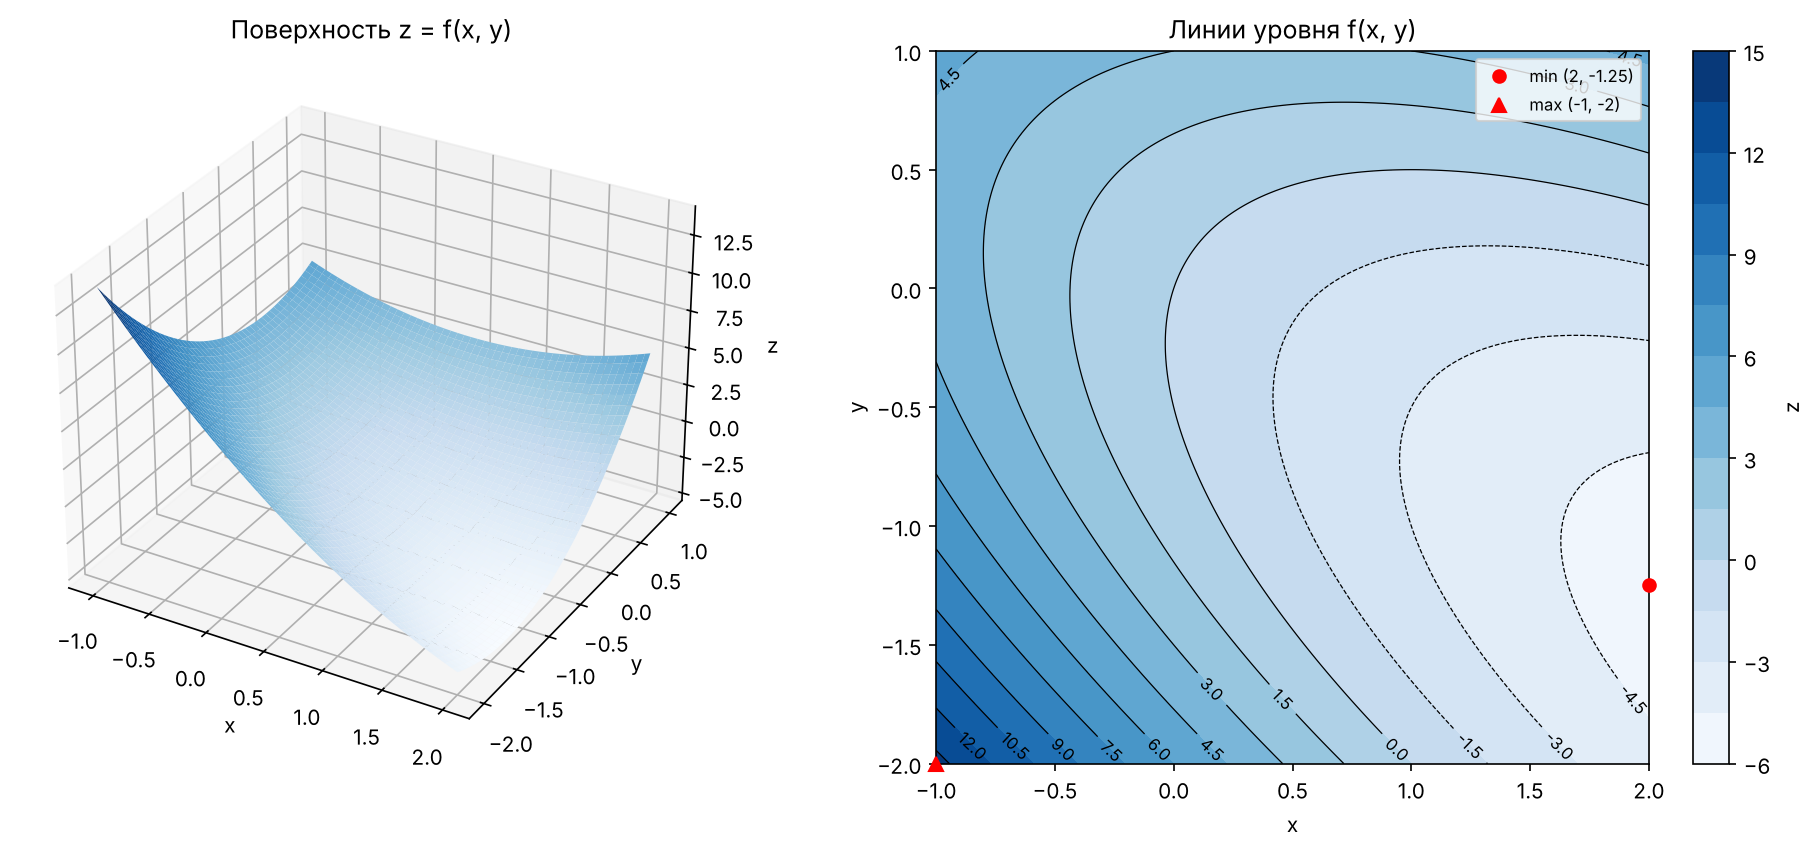
\includegraphics[width=\textwidth]{f3_plot.png}
\caption{Поверхность $z=f_3(x,y)$ (слева) и линии уровня (справа) на брусе $X=[-1,2]\times[-2,1]$; отмечены точки минимума и максимума на $X$.}
\label{fig:f3}
\end{figure}

\textbf{E.2.} Градиент $\nabla f_3=(2x+2y-3,\ 2x+4y+1)$ обращается в нуль в точке $(3.5,\,-2)\notin X$. Гессиан $\begin{pmatrix}2&2\\2&4\end{pmatrix}$ положительно определён ($2>0$, $\det=4>0$), поэтому $f_3$ выпукла. Так как стационарная точка лежит вне бруса, минимум достигается на границе, а максимум "--- в одной из вершин. Значения в вершинах: $f_3(-1,-2)=14$, $f_3(-1,1)=5$, $f_3(2,-2)=-4$, $f_3(2,1)=5$. Минимумы на рёбрах (на каждом ребре $f_3$ "--- квадратичная функция одной переменной):
\[
\begin{aligned}
x=-1:&\quad 2y^2-y+4, && \min \text{ при } y=\tfrac14:\ 3.875;\\
x=2:&\quad 2y^2+5y-2, && \min \text{ при } y=-\tfrac54:\ -5.125;\\
y=-2:&\quad x^2-7x+6, && \min \text{ при } x=2:\ -4;\\
y=1:&\quad x^2-x+3, && \min \text{ при } x=\tfrac12:\ 2.75.
\end{aligned}
\]
Итак, $\ran(f_3,X)=[f_3(2,-1.25),\ f_3(-1,-2)]=[-5.125,\ 14]$, $\rad=9.5625$.

\textbf{E.3--E.8.} Естественное расширение (E.3):
\[
X_1^2+2X_1X_2+2X_2^2-3X_1+X_2=[0,4]+[-8,4]+[0,8]+[-6,3]+[-2,1]=[-16,20].
\]
Эквивалентные выражения (E.4) получены выделением полных квадратов в разном порядке:
\begin{align*}
f_3(x,y)&=\tfrac12\bigl(x-\tfrac72\bigr)^2+2\bigl(y+\tfrac x2+\tfrac14\bigr)^2-\tfrac{25}{4}\\
&=\bigl(x+y-\tfrac32\bigr)^2+(y+2)^2-\tfrac{25}{4}\\
&=(x+y)^2+y^2-3x+y.
\end{align*}
Первая запись получена выделением квадрата сначала по $y$, затем по $x$; вторая "--- сначала по $x$. Частные производные линейны, и каждая переменная входит в них один раз, поэтому их естественные расширения точны: $\partial f_3/\partial x\in[-9,3]$, $\partial f_3/\partial y\in[-9,9]$. Для E.5 взяты центры $c=\Mid X=(0.5,\,-0.5)$, $c=(0,0)$ и вершина $c=(-1,-2)$. Для бицентрированной формы (E.6) $p=(-0.5,\ 0)$, $c_{*}=(1.25,\,-0.5)$, $c^{*}=(-0.25,\,-0.5)$; $F_{mv}(X,c_{*})=[-23.688,\ 30.313]$, $F_{mv}(X,c^{*})=[-32.688,\ 21.313]$. При дроблении (E.7) брус делится пополам по одной переменной ($[-1,0.5]\cup[0.5,2]$ по $x$ или $[-2,-0.5]\cup[-0.5,1]$ по $y$), естественное расширение вычисляется на каждой половине, и берётся оболочка результатов:
\begin{align*}
\text{по } x&:\quad \square\bigl([-5.5,\,17]\cup[-15.75,\,15.5]\bigr)=[-15.75,\,17],\\
\text{по } y&:\quad \square\bigl([-15.5,\,18.5]\cup[-8.5,\,14]\bigr)=[-15.5,\,18.5].
\end{align*}
Покоординатная липшицевская оценка (E.8): $L_1=\Mag[-9,3]=9$, $L_2=\Mag[-9,9]=9$, $L_1\rad X_1+L_2\rad X_2=9\cdot1.5+9\cdot1.5=27$. Сравнение всех оценок (E.9) приведено в табл.~\ref{tab:f3}.

\begin{table}[H]
\centering
\begin{tabular}{|l|c|c|c|}
\hline
Метод & $F(X)$ & $\rad F$ & $\dist(F,\ran)$ \\
\hline
\textbf{E.4:} $\frac12(x-\frac72)^2+2(y+\frac x2+\frac14)^2-\frac{25}4$ & $[-5.125,\ 14.000]$ & 9.563 & \textbf{0.000} \\
E.4: $(x+y)^2+y^2-3x+y$ & $[-8.000,\ 17.000]$ & 12.500 & 3.000 \\
E.4: $(x+y-\frac32)^2+(y+2)^2-\frac{25}4$ & $[-6.250,\ 23.000]$ & 14.625 & 9.000 \\
E.7: дробление по $y$ & $[-15.500,\ 18.500]$ & 17.000 & 10.375 \\
E.7: дробление по $x$ & $[-15.750,\ 17.000]$ & 16.375 & 10.625 \\
E.3: естественное расширение & $[-16.000,\ 20.000]$ & 18.000 & 10.875 \\
E.6: бицентрированная & $[-23.688,\ 21.313]$ & 22.500 & 18.563 \\
E.5: $F_{mv}$, $c=\Mid X=(0.5,-0.5)$ & $[-28.750,\ 25.250]$ & 27.000 & 23.625 \\
E.5: $F_{mv}$, $c=(0,0)$ & $[-36.000,\ 27.000]$ & 31.500 & 30.875 \\
E.5: $F_{mv}$, $c=(-1,-2)$ (вершина) & $[-40.000,\ 50.000]$ & 45.000 & 36.000 \\
\hline
\end{tabular}
\caption{Сравнение оценок для $f_3$ ($\ran=[-5.125,\ 14]$, $\rad=9.5625$)}
\label{tab:f3}
\end{table}

\textbf{Наблюдения:}
\begin{itemize}
\item \textbf{Лучший результат по $\dist$} "--- запись $\frac12(x-\frac72)^2+2(y+\frac x2+\frac14)^2-\frac{25}4$: оценка совпадает с точной областью значений ($\dist=0$). Переменная $x$ входит в неё дважды, но завышения не возникает: первое слагаемое зависит только от $x$ и принимает на $X_1$ значения $[1.125,\ 10.125]$ (минимум при $x=2$, максимум при $x=-1$), а второе "--- значения $[0,\ 10.125]$, причём минимум $0$ достигается при $x=2$, $y=-1.25\in X_2$, а максимум "--- при $x=-1$, $y=-2$. Экстремумы обоих слагаемых достигаются в одних и тех же точках бруса, совпадающих с точками минимума и максимума $f_3$.
\item \textbf{Запись $(x+y)^2+y^2-3x+y$} даёт $\dist=3$: минимумы слагаемых достигаются в несовместных точках ($x+y=0$, $y=0$, $x=2$, $y=-2$), как и максимумы ($x+y=\pm3$, $y=-2$, $x=-1$, $y=1$).
\item \textbf{Запись $(x+y-\frac32)^2+(y+2)^2-\frac{25}4$} даёт $\dist=9$, т.\,е. лишь немного лучше естественного расширения. Оба квадрата обращаются в нуль одновременно только в стационарной точке $(3.5,\,-2)$, лежащей вне бруса, поэтому нижняя граница $-6.25$ "--- это безусловный минимум, недостижимый на $X$. Верхняя граница $23$ ещё хуже: максимумы квадратов ($20.25$ при $(-1,-2)$ и $9$ при $y=1$) достигаются в разных точках. Таким образом, для одной и той же функции порядок выделения квадратов меняет результат от точного до почти не улучшающего оценку.
\item \textbf{Дробление} улучшает естественное расширение незначительно: по $y$ "--- $\dist$ с 10.875 до 10.375, по $x$ "--- до 10.625. Обе переменные входят в выражение трижды ($x$: $x^2$, $2xy$, $-3x$; $y$: $2xy$, $2y^2$, $y$), и обе границы естественного расширения формируются несовместными значениями обеих переменных: верхняя граница $20=4+4+8+3+1$ требует $x=2$ и $x=-1$, $y=-2$ и $y=1$, нижняя $-16=0-8+0-6-2$ "--- $x=0$ и $x=2$, $y=0$ и $y=-2$. Разрез по $x$ разносит $x=-1$ и $x=2$ по разным половинам и заметно снижает верхнюю границу (до 17), но почти не меняет нижнюю ($-15.75$), которая и определяет $\dist$. Разрез по $y$ меньше улучшает верхнюю границу (18.5), но чуть сильнее "--- нижнюю ($-15.5$), поэтому по $\dist$ он немного лучше, а по ширине "--- немного хуже.
\item \textbf{Бицентрированная форма} ($\dist=18.563$) лучше всех дифференциальных форм, но в 1.7 раза хуже естественного расширения.
\item \textbf{Дифференциальные центрированные формы} "--- худшие результаты ($\dist$ от 23.625 до 36), хотя оценки производных здесь точные: производные меняются в широком диапазоне (ширины 12 и 18) и умножаются на $X_i-c_i$ ширины 3. Центр $\Mid X$ даёт и минимальную полуширину (27, в согласии с теоремой Баумана), и минимальное $\dist$ среди рассмотренных центров, однако эта форма симметрична относительно $f_3(\Mid X)=-1.75$, тогда как середина $\ran$ равна $4.4375$. Центр в вершине бруса "--- худший.
\item \textbf{Покоординатная липшицевская оценка} (E.8) выполняется: $\rad F=18\le27$ для естественного расширения и $\rad\ran=9.5625\le27$. Для $F_{mv}(X,\Mid X)$ она выполняется как равенство ($\rad=27$): при центре в середине бруса $\rad\bigl(\mathbf{D}_i(X_i-c_i)\bigr)=\Mag\mathbf{D}_i\cdot\rad X_i$, а $\Mag\mathbf{D}_i=L_i$, поскольку оценки производных $\mathbf{D}_i$ точные.
\end{itemize}

% ======================= 5. Обсуждение =======================
\section{Обсуждение}

\subsection*{Влияние формы функционального выражения}
Форма выражения оказалась главным фактором точности. Для $f_1$ схема Горнера уменьшила ширину оценки вдвое (с 54 до 27) и сделала точной верхнюю границу, но $\dist$ уменьшилось лишь с 27 до 23, так как нижняя граница осталась прежней ($-25$). Для $f_2$ схема Горнера, напротив, ухудшила оценку ($[-24,18]$ против $[-16,20]$, $\dist$ 21.75 против 16): интервал $[-1,2]$ содержит нуль внутри, и произведение $X\cdot X$ шире квадрата $X^2$. Выделение полного квадрата дало точную область значений и для $f_2$, и для $f_3$; разложение $f_2$ на множители "--- промежуточный результат ($\dist=9.75$). Пример $f_3$ показывает, что важна не только идея преобразования, но и его конкретный вид: три эквивалентные записи дали $\dist=0$, 3 и 9. Общий принцип: выгодна запись, в которой переменные входят как можно меньше раз, а при нескольких вхождениях "--- такая, где экстремальные значения слагаемых достигаются в одной и той же точке бруса. Схема Горнера сама по себе улучшения не гарантирует.

\subsection*{Влияние выбора центра}
Для дифференциальной формы минимальная ширина достигается при $c=\Mid X$ (теорема Баумана); для $f_1$ "--- на всём отрезке $[c_{*},c^{*}]=[1.2,1.8]$, для $f_2$ "--- на $[c_{*},c^{*}]\approx[0.091,0.909]$. По $\dist$ середина оказалась лучшим из рассмотренных центров дифференциальной формы для всех трёх функций; однако для $f_3$ даже при этом центре форма смещена относительно $\ran$ (середины $-1.75$ и $4.4375$), т.\,е. важна не только ширина оценки, но и её положение относительно $\ran$. Центры на концах интервала (в вершине бруса) дали худшие результаты для дифференциальной формы у всех трёх функций. Для наклонной формы лучшие центры смещены от середины: $c=1.8$ для $f_1$ (6.8 против 9.5 при $c=1.5$) и $c=0.2$ для $f_2$ (13.590 против 16.625 при $c=0.5$).

\subsection*{Сравнение наклонной и дифференциальной форм}
При каждом из рассмотренных центров наклонная форма содержится в дифференциальной: $F_{sl}(X,c)\subseteq F_{mv}(X,c)$; для $f_1$ она уже в 3.6--5 раз, для $f_2$ "--- в 3.4--5.5 раза. Наклон $f^{\angle}(x,c)=f'(\xi)$ пробегает лишь часть значений производной, а его оценка по сокращённой дроби оказывается значительно уже естественного расширения производной (для $f_1$ при $c=1.5$: $[-6.75,2.25]$ против $[-18,27]$; для $f_2$ при $c=0.5$: $[-11.875,2.375]$ против $[-24,42]$). Для $f_2$ наклонная форма "--- единственная из центрированных, которая при удачном центре точнее естественного расширения (13.590 против 16). При этом на точность наклонной формы влияет и способ вычисления самого наклона: частное по схеме Горнера дало бы для $f_2$ лишь $\dist=21.510$.

\subsection*{Центрированные формы на широких интервалах}
Для всех трёх функций дифференциальные формы и бицентрированная форма оказались хуже естественного расширения. Причин две. Во-первых, интервалы широкие ($\wid X=3$), а квадратичный порядок приближения центрированных форм даёт выигрыш лишь при малой ширине. Во-вторых, для $f_1$ и $f_2$ естественное расширение производной сильно завышено: $[-18,27]$ вместо $[-3,9]$ и $[-24,42]$ вместо $[-6.086,12]$, и это завышение умножается на $X-c$. Для $f_3$ оценки частных производных точные, но сами производные меняются в широком диапазоне, и слагаемые $\mathbf{D}_i(X_i-c_i)$ получаются шире естественного расширения.

\subsection*{Бицентрированная форма}
Теорема Баумана подтверждается численно: для $f_1$ нижняя граница бицентрированной формы совпадает с наилучшей нижней границей среди $F_{mv}(X,c)$ (при $c=1.2=c_{*}$), верхняя "--- с наилучшей верхней (при $c=1.8=c^{*}$); для $f_2$ центры $c_{*}\approx0.091$, $c^{*}\approx0.909$ не попадают в сетку, и границы $F_{bic}$ строго лучше всех границ табл.~\ref{tab:f2c}; для всех трёх функций $F_{bic}$ содержится в каждой из вычисленных форм $F_{mv}$. Однако теорема оптимизирует центр внутри класса дифференциальных форм и не устраняет их главный недостаток "--- ширину оценки производной. Поэтому бицентрированная форма остаётся хуже естественного расширения ($\dist=30.992$, $42.369$, $18.563$ против 27, 16, 10.875). Гарантированно точный результат она даёт при $0\notin\bff'(X)$, что здесь не выполняется: оценки производных всех трёх функций содержат нуль.

\subsection*{Липшицевы оценки}
Неравенство $\rad F(X)\le L\rad X$ с константой Липшица самой функции для естественного расширения не гарантировано: для $f_1$ оно нарушается в 2 раза, для $f_2$ выполняется как равенство (18 = 18). Корректная оценка для расширения использует его собственную константу $L_F\ge L$ и выполняется для обеих функций с запасом. Для $f_3$ покоординатная оценка (27) выполняется ($\rad F=18$) и совпадает с полушириной дифференциальной формы с центром в середине бруса.

\subsection*{Дробление бруса}
Для $f_3$ однократное дробление бруса пополам дало лишь небольшое улучшение: по $y$ "--- $\dist$ с 10.875 до 10.375, по $x$ "--- до 10.625. Обе переменные входят в выражение по три раза и участвуют в формировании обеих завышенных границ, поэтому один разрез устраняет только часть несовместных комбинаций значений. Разрез по $x$ сильнее сужает оценку в целом (верхняя граница 17 против 18.5), а разрез по $y$ немного лучше приближает нижнюю границу, которая определяет $\dist$. Выбор переменной для дробления, таким образом, зависит от критерия качества, а выигрыш от одного разреза мал по сравнению с выбором удачной записи функции ($\dist=0$ для первого выражения с полными квадратами).

% ======================= 6. Выводы =======================
\section{Выводы}
\begin{enumerate}
\item Реализованы и сравнены по расстоянию $\dist(F,\ran)$ естественное расширение, форма Горнера, выделение полного квадрата и разложение на множители, дифференциальная и наклонная центрированные формы с разными центрами, бицентрированная форма (теорема Баумана), дробление бруса и липшицевы оценки.
\item Найдены точные области значений: $f_1$ на $[0,3]$: $[-2,2]$; $f_2$ на $[-1,2]$: $[-2.25,\ 4]$; $f_3$ на $[-1,2]\times[-2,1]$: $[-5.125,\ 14]$.
\item Для $f_1$ наилучший результат "--- наклонная форма при $c=1.8$ ($\dist=6.8$), далее форма Горнера (23) и естественное расширение (27); бицентрированная (30.992) и дифференциальные формы ($\ge39.875$) хуже естественного расширения.
\item Для $f_2$ выделение полного квадрата $\bigl(x^2-\frac52\bigr)^2-\frac94$ даёт точную область значений ($\dist=0$), разложение на множители "--- $\dist=9.75$, наклонная форма при $c=0.2$ "--- 13.590, естественное расширение "--- 16. Схема Горнера для $f_2$ хуже исходной записи (21.75), так как интервал содержит нуль внутри.
\item Для $f_3$ выражение $\frac12(x-\frac72)^2+2(y+\frac x2+\frac14)^2-\frac{25}4$ даёт точную область значений ($\dist=0$), тогда как другой порядок выделения квадратов "--- лишь $\dist=9$; дробление по $y$ и по $x$ слабо улучшает естественное расширение (10.375 и 10.625 против 10.875); дифференциальные и бицентрированная формы ($\dist\ge18.563$) значительно хуже естественного расширения.
\item Наклонная форма при каждом центре содержится в дифференциальной с тем же центром и уже её в 3.4--5.5 раза; для $f_2$ при удачном центре она точнее естественного расширения. Точность наклонной формы зависит от способа вычисления наклона.
\item Бицентрированная форма, в согласии с теоремой Баумана, содержится в каждой дифференциальной форме, но на широких интервалах и при завышенной оценке производной проигрывает естественному расширению.
\item Оценка $\rad F(X)\le L\rad X$ через константу Липшица функции для естественного расширения не гарантирована (для $f_1$ нарушается в 2 раза, для $f_2$ выполняется как равенство); оценка через константу расширения $L_F$ выполнена для $f_1$ и $f_2$, покоординатная липшицевская оценка для $f_3$ также выполнена.
\end{enumerate}

% ======================= 7. Список литературы =======================
\section{Список литературы}
\begin{enumerate}
\item А.Н. Баженов, А.А. Карпова «Интервальный анализ в примерах». "--- СПбПУ, 2024.
\item Документация NumPy "--- \url{https://numpy.org/doc/}
\item Документация Matplotlib "--- \url{https://matplotlib.org/}
\item Библиотека intvalpy "--- \url{https://pypi.org/project/intvalpy/}
\end{enumerate}

% ======================= 8. Приложение =======================
\section{Приложение}
Ссылка на репозиторий с исходным кодом (\texttt{calculations.py}, \texttt{plots.py}, \texttt{results.py}):\\
\url{https://github.com/USERNAME/REPOSITORY}

\end{document}
